\documentclass[british]{beamer}

\usepackage{default}
\usepackage[british]{babel}
\usepackage{epstopdf}
\usetheme{Madrid}
\usepackage{graphicx}
\usepackage{dirtytalk}
\usepackage{csquotes}
\usepackage{wrapfig}
\usepackage{tikz}
\usepackage{smartdiagram}
\usepackage{amsmath}
\usepackage{hyperref}


\begin{document}
%
\title[Big Data Project]
{Big Data Project}

\subtitle{Hertfordshire and North London Water Quality}

\author[F. Picciotti (matr.854021)]
{Francesco Picciotti (matr. 854021)}

%\date{23rd May 2017}

\institute[PoliMi]
{
	Politecnico di Milano
}

\logo{
	
\includegraphics[height=1.6cm,trim={0 2cm 4.5cm 2cm},clip]
	{./Imgs/Politecnico-di-Milano-3-m8qw.eps}
	}

\AtBeginSection[]
{
	\begin{frame}
		\frametitle{Outline}
		\tableofcontents[currentsection, currentsubsection]
	\end{frame}
}

\AtBeginSubsection[]{
	\begin{frame}
		\frametitle{Outline}
		\tableofcontents[currentsection, currentsubsection]
	\end{frame}
}

\maketitle

\section{Data Exploration}

\begin{frame}{Original Dataset}
	The original dataset contains 361101 samples (tuples) taken in the area nearby the Herfordshire and North London during a time span that goes from 2009 to 2016.
	
	The measurements are sampled by the UK Environment Agency and other datasets are available
	\href{http://environment.data.gov.uk/water-quality/view/download}{\textbf{here}}.
	Each tuple has the following fields:
	\begin{columns}
	\column{0.8\textwidth}
	\begin{itemize}
		\item \textbf{\_c0}: It's the row index, thus a progressive number
		\item \textbf{@id}: URI identifier
		\item \textbf{sample.samplingPoint}: The URI for making reference to a sampling point
		\item \textbf{sample.samplingPoint.notation}: A shorten string identifing each sampling point e.g.TH-PBRE9999
		\item \textbf{sample.samplingPoint.label}: The full name of the sampling point
		\item \textbf{sample.sampleDateTime}: The date and time when a sample was collected
	\end{itemize}
	\end{columns}
\end{frame}

\begin{frame}{Tuples' Features cont.}
	\begin{columns}
		\column{0.8\textwidth}
		\begin{itemize}
		\item \textbf{determinand.label}: A brief string identifing the determinand sampled, which is the property measured
		\item \textbf{determinand.definition}: A string describing the determinand meaning, its definition
		\item \textbf{determinand.notation}: A string which uniquely identifies the determinand
		\item \textbf{resultQualifier.notation}: This feature can be empty or containing "$<$","$>$" stating that is below or above the regulations
		\item \textbf{result}: The amount of the measured determinand
		\item \textbf{codedResultInterpretation.interpretation}: It is an empty column
		\item \textbf{determinand.unit.label}: The unit measure that expresses the \textbf{result} field
		\end{itemize}
	\end{columns}
\end{frame}

\begin{frame}{Tuples' Features cont. II}
	\begin{columns}
		\column{0.8\textwidth}
		\begin{itemize}
			\item \textbf{sample.sampledMaterialType.label}: The kind of material (strech of water, matter, ecc.) from which the determinand is sampled
			\item \textbf{sample.isComplianceSample}: It is a boolean to indicate whether the sample has been collected for a compliance purpose
			\item \textbf{sample.purpose.label}: The string describing the kind of the sampling purpose
			\item \textbf{sample.samplingPoint.easting}: The easting of the point on the British National Grid
			\item \textbf{sample.samplingPoint.northing}: The northing of the point on the British National Grid 
		\end{itemize}
	\end{columns}
\end{frame}

\begin{frame}{Finding the most sampled pollutant...}
	\begin{itemize}
		\item In order to find the most sampled and problematic determinand (pollutant), the \href{https://en.wikibooks.org/wiki/Data_Mining_Algorithms_In_R/Frequent_Pattern_Mining/The_FP-Growth_Algorithm}{\textbf{FPGrowth algorithm}} is applied to the transactions grouped by sampling point and date.
		
		\item This frequent item algorithm yields \textbf{Ammonia(N)} as the most sapled, with a count of \textbf{17108} which is the 60\% of the transactions.
	\end{itemize}
\end{frame}

\begin{frame}{...and its reason!}
	By analyzing the ammonia samples, it was mostly present in:
	\begin{itemize}
		\item Sewage effluents (5129 times)
		\item River/Running Surface Water (11080 times)	
	\end{itemize}
	Which is the \textbf{95\%} (16209/17108) of the times!
	
	Especially the presence in the \textbf{river surface water} is meaningful since the Ammonia traces within water may come from:
	\begin{itemize}
		\item fertilizers
		\item food processing waste
		\item Industrial wastewater as non-conventional pollutant
	\end{itemize}
	
	The last two reasons can be both the reason since it implies the presence of industries, whereas the first cause would mean a high concentration  \\ of ammonia in the \textbf{undeground} water!.
\end{frame}
	
\section{Towards Time Series}

\begin{frame}{Original Time series}
	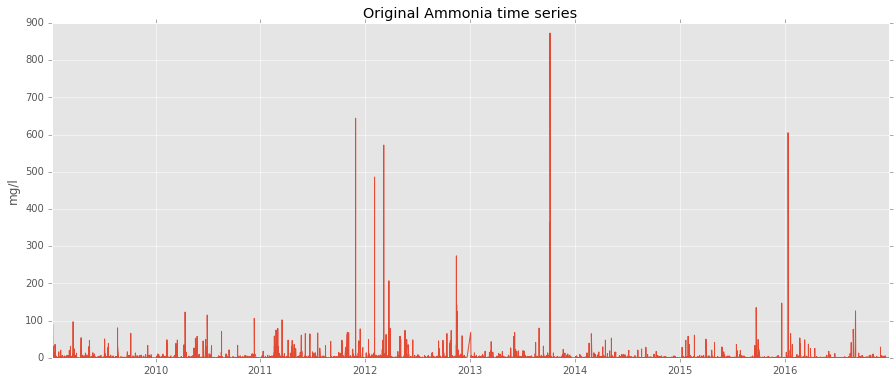
\includegraphics[width=1\textwidth]{./Imgs/original_ts.png}
\end{frame}

\subsection{Preprocessing}

\begin{frame}{Pipeline}
	\begin{center}
		\smartdiagramset{
			module minimum width= 5cm, 
			text width= 4.5cm,
			font= \tiny,
			set color list={blue!50!cyan,green!60!lime,orange!50!red,red!80!black},
			back arrow disabled=true}
		\smartdiagram[flow diagram: horizontal]{Outliers removal, Daily Resample and Imputation, Removing seasonal component, Transformation (with Box-Cox test), Scale between 0 and 1}
	\end{center}
\end{frame}

\subsection{Modeling and Validation}

\begin{frame}{ARMA Modeling}
	The \textbf{ARMA} model comes from statistics background.
	\begin{itemize}
		\item the AR is the \textbf{Autoregressive} part that takes in account of the previous steps equals to the AR's degree
		\item the MA is the \textbf{Moving Average} part that averages the stochastic side of the process equals to the MA's degree
	\end{itemize}
	Here, the \textbf{ARMA(2,1)} model is chosen by crossing two approaches:
	\begin{itemize}
		\item \textbf{AIC} (Akaike Information Criterion) and \textbf{BIC} (Bayesian Information Criterion) which are objective methods to select the degree that gives a good fit to the data preventing overfitting. This method computes gives the degree that enables the model to be enough complex to keep all the data's expressiveness
		\item \textbf{PACF} and \textbf{ACF}, the Partial AutoCorrelation Function and the AutoCorrelation Function are good indicators for finding out respectively the AR and MA degrees through a "elbow analysis".   
	\end{itemize}
\end{frame}

\begin{frame}{Validation I: Whiteness test (or Anderson Test) of the error}
	\begin{figure}
		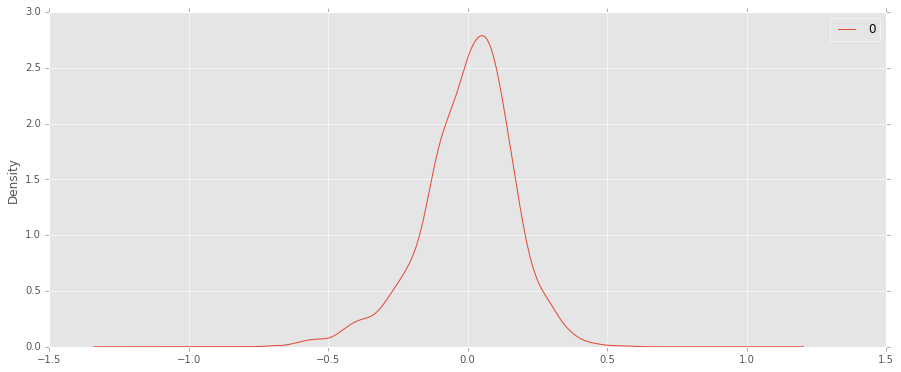
\includegraphics[width=\linewidth]{./Imgs/whiteness.png}
		\caption{The error distribution is close to a Gaussian with mean 0 and variance 1}
	\end{figure}
\end{frame}

\begin{frame}{Validation II: Out-sample performances evaluation}
		\begin{figure}
			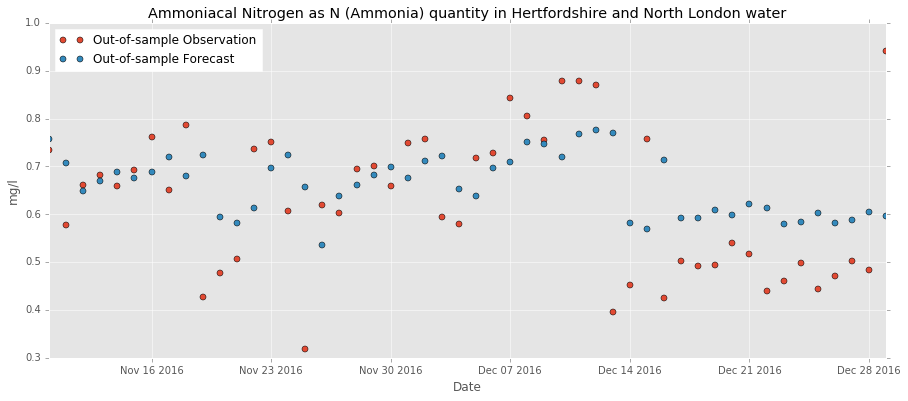
\includegraphics[width=\linewidth]{./Imgs/validation.png}
			\caption{Mean Squared Error: 0.019193}
		\end{figure}
\end{frame}
		
\section{References}

\begin{frame}{Guidelines}
	\begin{itemize}
		\item \href{https://spark.apache.org/docs/2.1.0/api/python/}{\textbf{Spark and Pyspark doc}}
		\item Spark understanding and basic knowledge from Big Data part held by prof. Ardagna during the Computing Infrastructures course @ Polimi
		\item \href{http://www.statsmodels.org/stable/index.html}{\textbf{Statsmodels}}: python module and its doc 
		\item Notes from Model Identification and Data Analysis (MIDA/IMAD) course @ Polimi by prof. Bittanti and Savaresi
		\item \href{http://people.duke.edu/~rnau/411home.htm}{\textbf{Statistical forecasting}}: notes on regression and time series analysis by Robert Nau (Fuqua School of Business, Duke University) 
		\item \href{https://stats.stackexchange.com/}{\textbf{Cross Validated}}: Stack Overflow for stats guys in trouble
	\end{itemize}
\end{frame}

\end{document}
